\chapter{Visualizing Dynamic Input Graphs}
\label{chap:visualizing-dynamic-input-graphs}

Extending the approach discussed in the previous section to dynamic input graphs is challenging primarily because we must try to preserve the viewer's mental map as the underlying data changes over time.
We want the visualization at different points in time to be similar enough so that the viewer can clearly tell what parts have changed \cite{mashima2011visualizing}, yet allow for the required changes in geography and topology.
Still, changes between visualizations at consecutive points in time should minimize movement and allow for smooth animations therebetween.

Extending the pipeline for static inputs discussed in the previous section in a straightforward way will not satisfy these requirements.
Running through the entire pipeline with a different, albeit similar, input graph, may result in a completely different visualization, destroying the viewer's mental map.
This is because even though the combinatorial arrangement of regions in the map \propmap{t} is predetermined by the planar embedding of the filtered cluster graph \clustergraph{t}, the independent nature of the runs through the pipeline can result in regions with drastically different shapes and (absolute) positions.
We therefore extend the pipeline in a way that allows for small, incremental changes to be propagated through the pipeline and to eventually be applied to the previous output in a way that preserves the viewer's mental map.

We extend the pipeline for static input by an incremental transformation phase.
This phase takes two inputs:
A map \initmap{t} that the pipeline previously produced as output for some filtered cluster graph \clustergraph{t}, and a sequence of operations on said cluster graph, that, when applied to \clustergraph{t}, yields the cluster graph \clustergraph{t+1}.
The incremental transformation phase then determines how these operations translate to a polygonal dual of \clustergraph{t} and applies the translated operations to \initmap{t}, producing \initmap{t+1}, a polygonal dual of \clustergraph{t+1}.
This new polygonal dual is then fed back into the drawing phase to make it an $\varepsilon$-area-proportional contact representation \propmap{t+1} for some small $\varepsilon > 0$ and to improve the local fatness of the map's regions.

\begin{figure}[H]
	\centering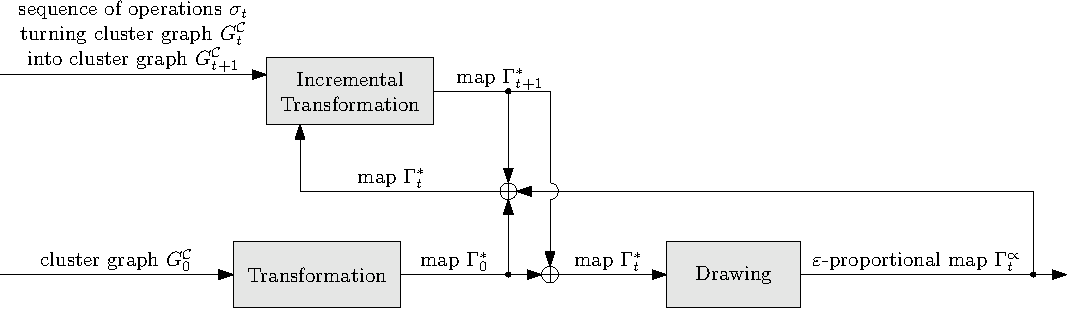
\includegraphics[width=0.9\textwidth]{Resources/Framework-3.pdf}
	\caption{Overview of the algorithmic pipeline for dynamic input graphs.}
	\label{fig:dynamic-pipeline-thesis}
\end{figure}

Real-world applications, such as visualizing a dynamic opinion network, need a way to feed a sequence of operations on the filtered cluster graph into our framework.
This could be done by prepending an incremental clustering phase that translates changes to the simple input graph $G_t$ into changes of its filtered cluster graph \clustergraph{t}.
However, such a sequence of operations $\sigma_t$ is only meaningful in combination with a graph that these operations can be applied to.
One must therefore provide the previously-produced cluster graph \clustergraph{t} as additional input to the incremental clustering phase such that it can tailor its output to the cluster graph that has already been locked in in an earlier run through the pipeline.
This possible extension to our pipeline is illustrated in the following figure:
%
\begin{figure}[H]
	\centering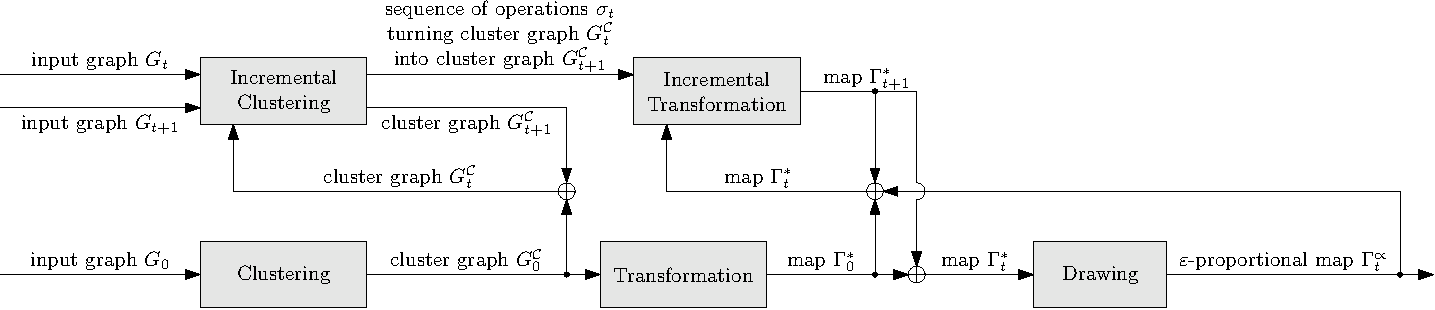
\includegraphics[width=\textwidth]{Resources/Framework-4.pdf}
	\caption{Overview of a possible algorithmic pipeline for generic applications.}
	\label{fig:dynamic-pipeline-application}
\end{figure}

Extending the pipeline to allow the propagation of small, incremental changes of the input graph has numerous benefits other than the ability to preserve the viewer's mental map:
%
\begin{itemize}
\item It allows highly efficient implementations of the incremental parts of the pipeline as only the aspects that have actually changed in the input graph or intermediate products need to be processed and propagated further along the pipeline.
\item It makes the dynamic pipeline highly parallelizable: when a later phase is processing changes, an earlier phase can already start processing new changes independently.
With our force-directed implementation of the drawing phase, we can even incorporate dynamic updates while the drawing phase is still running, even if it has not converged yet: we pause the force simulation, feed the current map \initmap{t} into the incremental transformation phase to incorporate the dynamic updates, and then resume the simulation with the updated map graph \initmap{t+1} produced by the incremental transformation phase.
\item It efficiently supports dynamic input in an online setting, \ie{} a setting in which the incremental changes aren't known in advance, for example when visualizing live data.
\end{itemize}



\paragraph{Supported Operations}

Our pipeline supports numerous classes of primitive operations on the filtered cluster graph, such as inserting and removing vertices and edges, flipping edges, or simply changing a cluster's weight.
By composing multiple primitive operations in a sequence, more drastic changes can be made to the filtered cluster graph.
In our pipeline, the operations are applied one after the other nonetheless.

The simplest operation of all is changing a vertex $v$'s weight:
We simply take the previous $\varepsilon$-proportional map \propmap{t}, update the weight of the face $f_v$ corresponding to the vertex $v$, and declare that as the new map \initmap{t+1}.
The map \initmap{t+1} then runs through the drawing phase again to account for the updated face weights.

Implementing the remaining operations as part of the incremental transformation is a little more challenging, and we'll discuss those in great detail in the following sections.

\clearpage
\section{Inserting Vertices}
\label{sect:inserting-vertices}

When a new cluster appears in our underlying data set, we want to add a new vertex to the cluster graph. We distinguish between adding a new vertex on the inside and adding a new vertex on the outside because different rules apply.



\paragraph{Inserting Vertices Inside}

All internal faces of the cluster graph are triangles. If we add a vertex in one of the triangular faces, we must also add edges to the three vertices bounding the face without introducing edge crossings in order to preserve the graph's internal triangulatedness. A valid vertex insertion into an internal face is illustrated in \cref{fig:insert-vertex-inside-example}.

\begin{figure}[H]
	\centering
	\subfigure[]{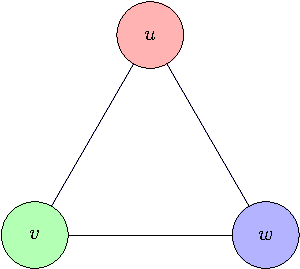
\includegraphics[height=29mm]{Resources/InsertVertexInside-Example-1.pdf}}
	\quad
	\subfigure[]{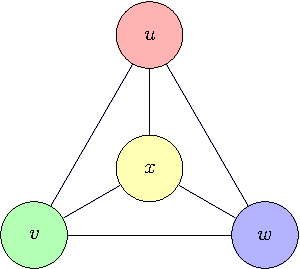
\includegraphics[height=29mm]{Resources/InsertVertexInside-Example-2.pdf}}
	\qquad
	\subfigure[]{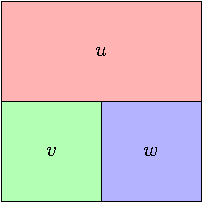
\includegraphics[height=29mm]{Resources/InsertVertexInside-Example-3.pdf}}
	\quad
	\subfigure[]{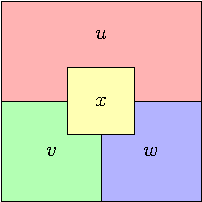
\includegraphics[height=29mm]{Resources/InsertVertexInside-Example-4.pdf}}
	\caption{A cluster graph and a polygonal dual thereof, before (a, c) and after (b, d) inserting the vertex $x$ in the triangular face $uvw$.}
	\label{fig:insert-vertex-inside-example}
\end{figure}

Let $u$, $v$, and $w$ be the vertices bounding an internal face of the cluster graph in counterclockwise order and $x$ the new vertex we want to add inside said face. We compute the paths that form the $u$-$v$-, $v$-$w$-, and $w$-$u$-boundaries in the polygonal dual. Let $p_{uvw}$ denote the vertex where the three faces corresponding to $u$, $v$, and $w$ meet. Let $p_{uv}$, $p_{vw}$, and $p_{wu}$ denote the first subdivision vertex on the boundary between faces $u$ and $v$, $v$ and $w$, and $w$ and $u$, respectively, starting from $p_{uwv}$. If one of the boundaries consist of only one edge, we place a subdivision vertex at its midpoint first. \Cref{subfig:insert-vertex-inside-illustration-1} shows how these vertices might look for the example from above.

\begin{figure}[H]
	\centering
	\subfigure[]{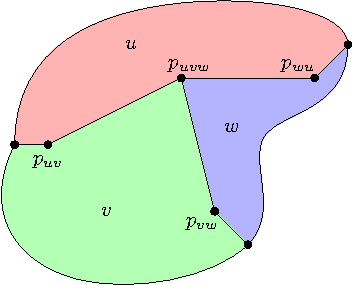
\includegraphics[width=45mm]{Resources/InsertVertexInside-Illustration-1.pdf}\label{subfig:insert-vertex-inside-illustration-1}}
	\quad
	\subfigure[]{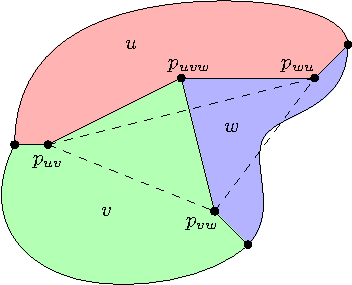
\includegraphics[width=45mm]{Resources/InsertVertexInside-Illustration-2.pdf}\label{subfig:insert-vertex-inside-illustration-2}}
	\quad
	\subfigure[]{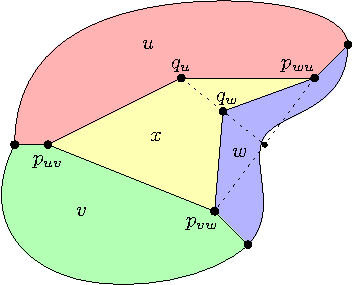
\includegraphics[width=45mm]{Resources/InsertVertexInside-Illustration-3.pdf}\label{subfig:insert-vertex-inside-illustration-3}}
	\caption{Inserting an internal face $x$ at the point where three faces $u,v,w$ meet.}
	\label{fig:insert-vertex-inside-illustration}
\end{figure}

Having determined the subdivision vertices $p_{uv}$, $p_{vw}$, and $p_{wu}$, we now want to remove the vertex $p_{uvw}$ and insert edges between the subdivision vertices instead to bound a new face for $d$ (dashed lines in \cref{subfig:insert-vertex-inside-illustration-2}). Doing so naïvely may introduce edge crossings and we generally need to add bends in the form of subdivision vertices to those edges. We distinguish three cases, all of which are illustrated in the figure:
%
\begin{itemize}
	\item If we can place an edge between $p_{ab}$ and $p_{bc}$ without introducing an edge crossing, we do not need to bend the edge (face $v$ in \cref{subfig:insert-vertex-inside-illustration-3}).
	\item Otherwise, if the internal angle of face $a$ at $p_{abc}$ is more than half a turn, we place the bend $q_a$ at $p_{abc}$ (face $u$ in \cref{subfig:insert-vertex-inside-illustration-3}).
	\item Otherwise we search for a bend location $q_a$ somewhere on the line segment from the midpoint of $p_{ab}$ and $p_{bc}$ to $p_{abc}$. We start at the midpoint of $p_{ab}$ and $p_{bc}$ and divide the remaining distance to $p_{abc}$ in half until we find a bend location for which the bent edge from $p_{ab}$ to $p_{bc}$ would not create edge crossings (face $w$ in \cref{subfig:insert-vertex-inside-illustration-3}).
\end{itemize}

Considering at most one angle at $p_{uvw}$ can be more than half a turn, we place at most one bend there. By removing the vertex $p_{uvw}$ and inserting the edges $\{p_{uv},p_{vw}\}$, $\{p_{vw},p_{wu}\}$, and $\{p_{wu},p_{uv}\}$, potentially with bends $p_v$, $p_w$, and $p_u$, we create an internal face for $x$.



\paragraph{Inserting Vertices Outside}

Alternatively, we can add a new vertex in the outer face of the cluster graph. Such a vertex must be connected to at least two vertices on the outer face to preserve the graph's 2-connectivity and its neighbors must form a path on the original boundary of the cluster graph in order not to create holes and thereby violate its internal triangulatedness.

We restrict ourselves to adding new vertices in the outer face that are made incident to exactly 2 neighboring vertices. Let $\{u,v\}$ be an edge on the outer face, then we support adding a new vertex $x$ in the outer face and connecting it to both $u$ and $v$. \Cref{fig:insert-vertex-outside-example} illustrates a valid vertex insertion into the outer face.

\begin{figure}[H]
	\centering
	\subfigure[]{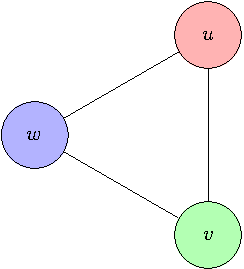
\includegraphics[height=29mm]{Resources/InsertVertexOutside-Example-1.pdf}}
	\quad
	\subfigure[]{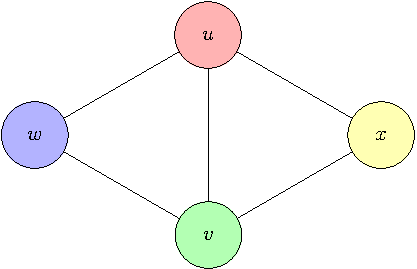
\includegraphics[height=29mm]{Resources/InsertVertexOutside-Example-2.pdf}}
	\qquad
	\subfigure[]{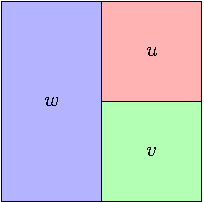
\includegraphics[height=29mm]{Resources/InsertVertexOutside-Example-3.pdf}}
	\quad
	\subfigure[]{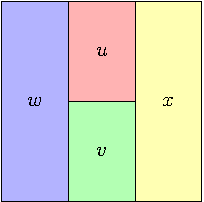
\includegraphics[height=29mm]{Resources/InsertVertexOutside-Example-4.pdf}}
	\caption{A cluster graph and a polygonal dual thereof, before (a, c) and after (b, d) inserting the vertex $x$ on the outer face and connecting it to $u$ and $v$.}
	\label{fig:insert-vertex-outside-example}
\end{figure}

Let $u$ and $v$ be the adjacent vertices on the outer face of the cluster graph and $x$ the new vertex we want to add in the outer face.
Let $p_{uv}$ denote the vertex where the faces $u$ and $v$ meet the outer face of the polygonal dual.
We define $p_u$ and $p_v$ as the first subdivision vertex we encounter when starting at $p_{uv}$ and following the boundary of $u$ and $v$ with the outer face, respectively.
If one of the boundaries consist of only one edge, we place a subdivision vertex at its midpoint and use that vertex as $p_u$/$p_v$.
\Cref{subfig:insert-vertex-outside-illustration-1} shows how these vertices might look for the example from above.
%

\begin{figure}[H]
	\centering
	\subfigure[]{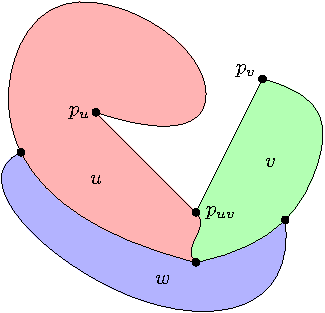
\includegraphics[width=45mm]{Resources/InsertVertexOutside-Illustration-1.pdf}\label{subfig:insert-vertex-outside-illustration-1}}
	\quad
	\subfigure[]{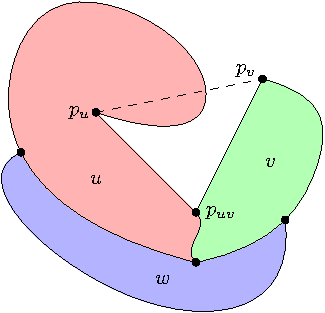
\includegraphics[width=45mm]{Resources/InsertVertexOutside-Illustration-2.pdf}\label{subfig:insert-vertex-outside-illustration-2}}
	\quad
	\subfigure[]{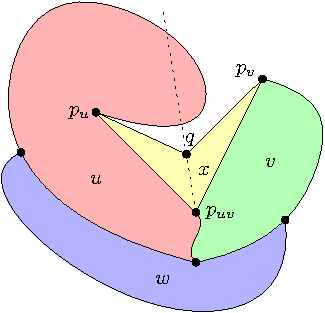
\includegraphics[width=45mm]{Resources/InsertVertexOutside-Illustration-3.pdf}\label{subfig:insert-vertex-outside-illustration-3}}
	\caption{Inserting a face $x$ at the point where the faces $u$ and $v$ meet the outer face.}
	\label{fig:insert-vertex-outside-illustration}
\end{figure}

With $p_u$ and $p_v$ determined, we can create the face $x$ by inserting a path to connect $p_u$ and $p_v$ without introducing edge crossings. Simply inserting an edge between $p_u$ and $p_v$ generally isn't enough, as illustrated in \cref{subfig:insert-vertex-outside-illustration-2}. However, with a single bend in the form of a subdivision vertex $q$, we can guarantee that no edge crossings are being created.

We search for a bend location on the outward-pointing bisector of the angle $\measuredangle_{p_up_{uv}p_v}$, starting at some fixed distance $\epsilon > 0$ and halving the distance until we find a valid location. As the possible bend location moves infinitesimally close to $p_{uv}$, we are guaranteed to find one that doesn't introduce edge crossings. By inserting a vertex at $q$ along with edges $\{q,p_u\}$ and $\{q,p_v\}$, we create an internal face for $x$, as illustrated in \cref{subfig:insert-vertex-outside-illustration-3}.

\clearpage
\section{Removing Vertices}
\label{sect:removing-vertices}

Clusters in the underlying data set can also fade and eventually cease to exist. In this case, we want to be able to remove existing vertices of the cluster graph. We make the same distinction here as when inserting vertices: we can remove internal vertices or vertices that lie on the cluster graph's outer face. 



\paragraph{Removing Internal Vertices}

When removing an internal vertex, we must ensure that the cluster graph remains internally triangulated. This is only the case if the vertex we want to remove has degree 3 as removing vertices with greater degree would create holes. If one wants to a vertex with degree 4 or higher, one must first tweak the adjacencies on the inside of the cluster graph using edge flips, discussed in \cref{sect:flipping-edges}. \Cref{fig:remove-vertex-example-internal} shows a valid removal of an internal vertex.

\begin{figure}[H]
	\centering
	\subfigure[]{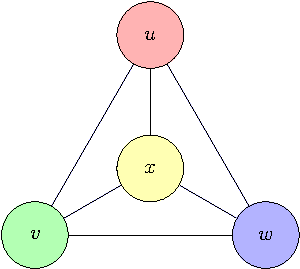
\includegraphics[height=29mm]{Resources/RemoveVertex-Example-Internal-1.pdf}}
	\quad
	\subfigure[]{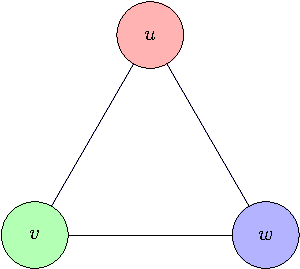
\includegraphics[height=29mm]{Resources/RemoveVertex-Example-Internal-2.pdf}}
	\qquad
	\subfigure[]{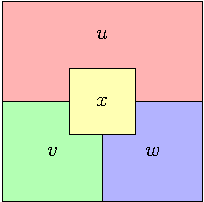
\includegraphics[height=29mm]{Resources/RemoveVertex-Example-Internal-3.pdf}}
	\quad
	\subfigure[]{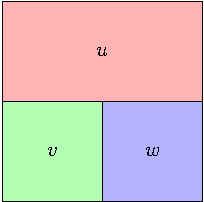
\includegraphics[height=29mm]{Resources/RemoveVertex-Example-Internal-4.pdf}}
	\caption{A cluster graph and a polygonal dual thereof, before (a, c) and after (d, d) removing the internal vertex $x$ with degree 3.}
	\label{fig:remove-vertex-example-internal}
\end{figure}

In order not to create holes in the contact representation, the incident faces must take over the area that the face to be removed originally occupied. Let $x$ denote the internal vertex we want to remove and $u$, $v$, and $w$ its three neighbors. We start by computing the paths that form the $u$-$v$-, $v$-$w$, and $w$-$u$-boundaries in the dual. Let $p_{uvx}$ ($p_{vwx}$, $p_{uwx}$) denote the vertex where face $x$ meets faces $u$ and $v$ ($v$ and $w$, $w$ and $u$). \Cref{subfig:remove-vertex-illustration-1} shows how these vertices might look for the example from above.

\begin{figure}[H]
	\centering
	\subfigure[]{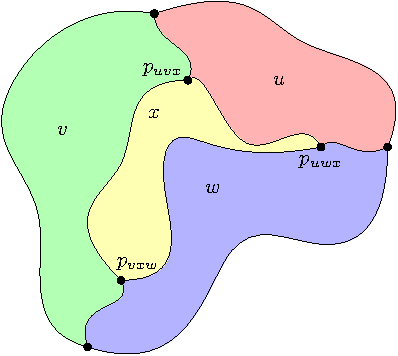
\includegraphics[width=45mm]{Resources/RemoveVertex-Illustration-1.pdf}\label{subfig:remove-vertex-illustration-1}}
	\quad
	\subfigure[]{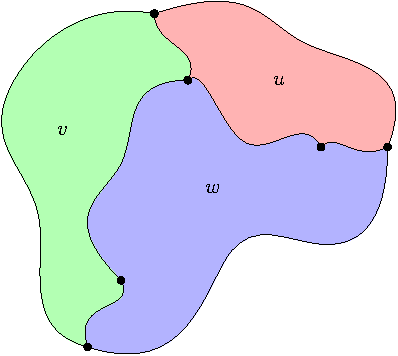
\includegraphics[width=45mm]{Resources/RemoveVertex-Illustration-2.pdf}\label{subfig:remove-vertex-illustration-2}}
	\caption{Removing an internal face $x$ incident to the faces $u$, $v$, and $w$.}
	\label{fig:remove-vertex-illustration}
\end{figure}

To remove the internal face $x$, we simply remove the its boundary to one of its neighboring faces. In doing so, the two faces effectively merge. In practice this works really well because large clusters don't disappear at a moment's notice, and small clusters generally occupy a very small area such that the operation is barely noticeable.




\paragraph{Removing External Vertices}

When removing vertices on the outer face along with its incident edges, we must ensure that the graph remains 2-connected afterwards. \cref{fig:remove-vertex-example-external} illustrates a valid removal of a vertex on the outer face. Similar to inserting vertices on the outer face, we restrict ourselves to removing vertices on the outer face that have degree 2. If we need to remove a vertex with higher degree, the additional edges need to be removed first as discussed in \cref{sect:flipping-edges}.

\begin{figure}[H]
	\centering
	\subfigure[]{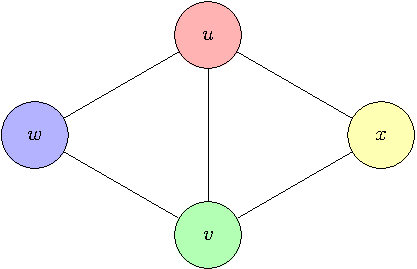
\includegraphics[height=29mm]{Resources/RemoveVertex-Example-External-1.pdf}}
	\quad
	\subfigure[]{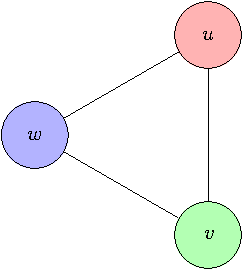
\includegraphics[height=29mm]{Resources/RemoveVertex-Example-External-2.pdf}}
	\qquad
	\subfigure[]{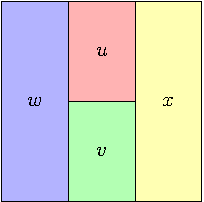
\includegraphics[height=29mm]{Resources/RemoveVertex-Example-External-3.pdf}}
	\quad
	\subfigure[]{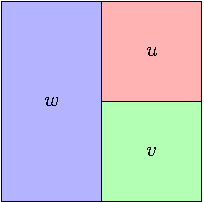
\includegraphics[height=29mm]{Resources/RemoveVertex-Example-External-4.pdf}}
	\caption{A cluster graph and a polygonal dual thereof, before (a, c) and after (b, d) removing the vertex $x$ on the outer face.}
	\label{fig:remove-vertex-example-external}
\end{figure}

This operation, too, is just a special case of the vertex removal discussed above. Referring to the construction of the augmented dual again, with the helper vertex $v^+$ and edges $\{v^+,\cdot\}$, removable vertices $x$ on the outer face of the cluster graph lie in a triangle formed by its two neighbors $u$ and $v$ and the helper vertex $v^+$.

The construction outlined above translates 1-to-1 to removing vertices from the outer face, except one of the three neighboring faces is the implicit outer face. In our implementation, we always remove the boundary of $x$ with the outer face and thereby transfer the area to the outer face.

\clearpage
\section{Flipping Edges}
\label{sect:flipping-edges}

Let us now discuss the edge flip mentioned in the previous sections.
An internal edge $\{u,v\}$ is incident to two different internal faces $f$, $g$.
Let $x$ and $y$ denote the third vertex bounding $f$ and $g$, respectively.
It is $x \neq y$ because the cluster graph is simple.
Flipping the edge $\{u,v\}$ would replace it with the edge $\{x,y\}$.
Consequently, this operation is only permitted iff $x$ and $y$ are not already adjacent \emdash{} otherwise, we would introduce a duplicate adjacency.
\Cref{fig:flip-edge-example-internal} shows an example of a valid edge flip operation.

\begin{figure}[H]
	\centering
	\subfigure[]{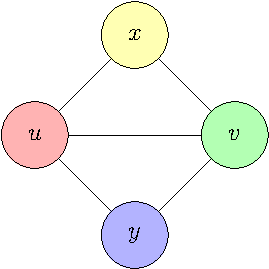
\includegraphics[height=28mm]{Resources/FlipEdge-Example-Internal-1.pdf}}
	\quad
	\subfigure[]{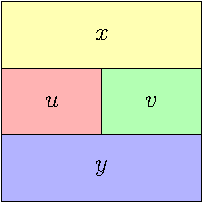
\includegraphics[height=28mm]{Resources/FlipEdge-Example-Internal-2.pdf}}
	\qquad
	\subfigure[]{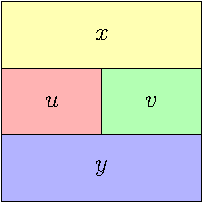
\includegraphics[height=28mm]{Resources/FlipEdge-Example-Internal-3.pdf}}
	\quad
	\subfigure[]{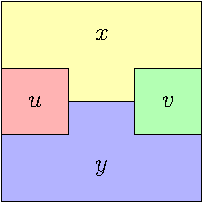
\includegraphics[height=28mm]{Resources/FlipEdge-Example-Internal-4.pdf}}
	\caption{A cluster graph and a polygonal dual thereof, before (a, c) and after (b, d) flipping the internal edge $\{u,v\}$.}
	\label{fig:flip-edge-example-internal}
\end{figure}

An edge flip in a cluster graph translates to region adjacencies being flipped in its dual.
Given a polygonal dual of some cluster graph, we apply an edge flip in two phases.
First, we contract the region boundary we want to remove into a single point, creating a degenerate contact representation in which four regions meet in a point.
In the second phase, we create a region boundary in the opposite direction, getting rid of the degeneracy at the point into which the original boundary has been contracted.

Let $u$ and $v$ be two adjacent faces in the polygonal dual whose boundary we want to contract.
Also, let path $P_{uv}$ be the maximal common boundary between $u$ and $v$, oriented such that $u$ lies on the left of it, and $v$ lies on the right of it.
At both endpoints of the path, $u$ and $v$ meet with a third face.
We denote the third face incident to the path's first vertex by $x$ and the third face incident to the path's last vertex by $y$, as illustrated in \cref{fig:flip-edge-example-internal}.
To contract the $u$-$v$-boundary into a single point, we repeatedly contract a peripheral edge on the boundary until the last edge has been contracted.
We do so on alternating ends, \ie{}, we start by contracting the first edge, then the last, then the first again, etc.

\begin{figure}[H]
	\centering
	\subfigure[]{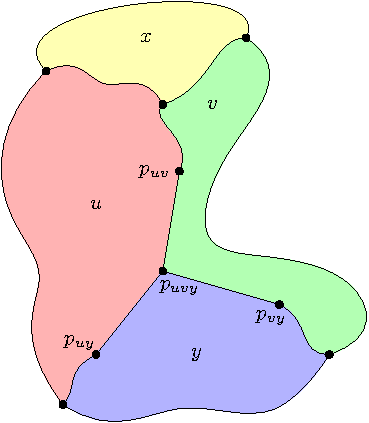
\includegraphics[width=40mm]{Resources/FlipEdge-ContractBoundaryBelow-1.pdf}\label{subfig:flip-edge-contract-boundary-below-1}}
	\quad
	\subfigure[]{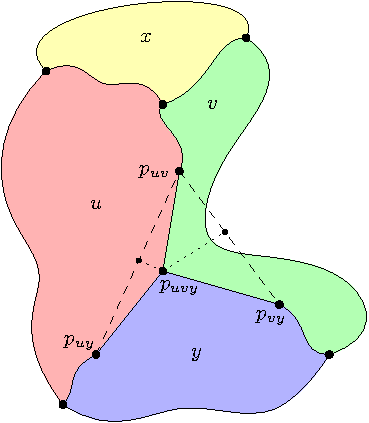
\includegraphics[width=40mm]{Resources/FlipEdge-ContractBoundaryBelow-2.pdf}\label{subfig:flip-edge-contract-boundary-below-2}}
	\quad
	\subfigure[]{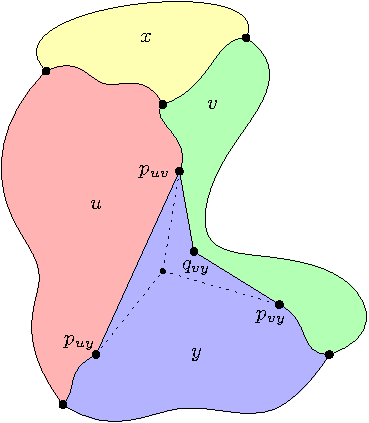
\includegraphics[width=40mm]{Resources/FlipEdge-ContractBoundaryBelow-3.pdf}\label{subfig:flip-edge-contract-boundary-below-3}}
	\caption{A contact representation before (a) and after (c) contracting the peripheral edge $\{p_{uv},p_{uvy}\}$ on the $u$-$v$-boundary away from $y$. (b) shows the construction of potential subdivision vertices.}
	\label{fig:flip-edge-contract-boundary-below}
\end{figure}

\Cref{fig:flip-edge-contract-boundary-below} illustrates how we contract the first edge of the oriented upwards without introducing edge crossings.
We describe only this construction in writing; the contraction of the last edge works virtually the same way and is illustrated in \cref{fig:flip-edge-contract-boundary-above}.
Let $p_{uvy}$ denote the vertex where the faces $u$, $v$, and $y$ meet and $p_{uy}$ and $p_{vy}$ the subdivision vertices on the $u$-$y$- and $v$-$y$-boundaries that are incident to $p_{uvy}$, respectively.
If the $u$-$y$- or $v$-$y$-boundary consists of only one edge, we subdivide it at its midpoint first.
Let $p_{uv}$ be the subdivision vertex on the $u$-$v$-boundary that is incident to $p_{uvy}$ or the last vertex of the oriented boundary if no such subdivision vertex exists.
To reduce the length of the $u$-$v$-boundary by one, we would want to remove $p_{uvy}$ and its incident edges and add edges from $p_{uv}$ to both $p_{uy}$ and $p_{vy}$.
These edges may introduce crossings, though, as illustrated by the dashed lines in \cref{subfig:flip-edge-contract-boundary-above-2} and \cref{subfig:flip-edge-contract-boundary-below-2}.
However, with just one bend on each of the edges, we can guarantee that no edge crossings are created:

\begin{itemize}
\item If adding the edge between $p_{uv}$ and $p_{ay}$ ($a \in \{u,v\}$) does not introduce a crossing, we simply add the edge.
(for $a = u$ in \cref{subfig:flip-edge-contract-boundary-below-2})
\item Otherwise, if the internal angle of face $a$ at $p_{uvy}$ is $180^\circ$ or more, we place the bend at $p_{uvy}$, \ie{}, we insert the edge $\{p_{uv},p_{ay}\}$ and subdivide it with a new vertex $q_{ay}$ at the position of $p_{uvy}$.
Note that at most one of the faces can have an internal angle at $p_{uvy}$ that is $180^\circ$ or more.
(for $a = v$ in \cref{subfig:flip-edge-contract-boundary-above-2})
\item Otherwise, we search for a bend location in the form of a subdivision vertex $q_{ay}$ somewhere on the outward-pointing bisector of the angle $\angle_{p_{ay}p_{uvy}p_{uv}}$ (dotted lines in \cref{subfig:flip-edge-contract-boundary-below-2} and \cref{subfig:flip-edge-contract-boundary-above-2}).
We start looking at the point where the bisector intersects the segment from $p_{uv}$ to $p_{ay}$ and repeatedly divide the remaining distance to $p_{uvy}$ in half until we find a bend location for which the bent edge from $p_{uv}$ to $p_{ay}$ would not introduce edge crossings.
As the candidate location moves infinitesimally close to $p_{uvy}$, we are guaranteed to find one that does not introduce crossings.
(for $a = v$ in \cref{subfig:flip-edge-contract-boundary-below-3} and $a = u$ in \cref{subfig:flip-edge-contract-boundary-above-3})
\end{itemize}

\begin{figure}[H]
	\centering
	\subfigure[]{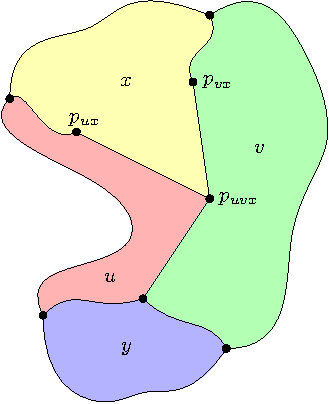
\includegraphics[width=40mm]{Resources/FlipEdge-ContractBoundaryAbove-1.pdf}\label{subfig:flip-edge-contract-boundary-above-1}}
	\quad
	\subfigure[]{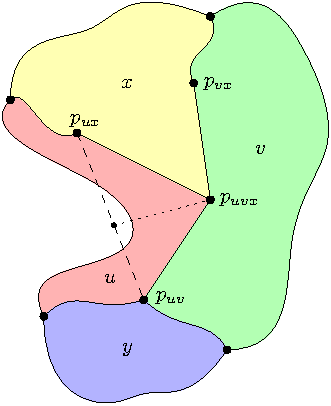
\includegraphics[width=40mm]{Resources/FlipEdge-ContractBoundaryAbove-2.pdf}\label{subfig:flip-edge-contract-boundary-above-2}}
	\quad
	\subfigure[]{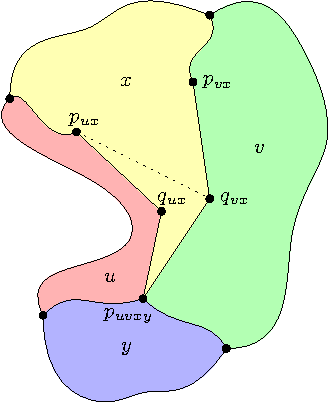
\includegraphics[width=40mm]{Resources/FlipEdge-ContractBoundaryAbove-3.pdf}\label{subfig:flip-edge-contract-boundary-above-3}}
	\caption{A contact representation before (a) and after (c) contracting the last remaining edge $\{p_{uvx},p_{uvy}\}$ on the $u$-$v$-boundary away from $y$. (b) shows the construction of potential subdivision vertices.}
	\label{fig:flip-edge-contract-boundary-above}
\end{figure}

Once the $u$-$v$-boundary has been contracted into a single vertex $p_{uvxy}$ where all four faces $u$, $v$, $x$, and $y$ now meet, as shown in \cref{subfig:flip-edge-contract-boundary-above-3}, we need to resolve the degeneracy and create a boundary in the opposite direction, \ie{}, an $x$-$y$-boundary.
Let $p_{ux}$, $p_{uy}$, $p_{vx}$, and $p_{vy}$ denote the subdivision vertices on the respective boundaries that are incident to $p_{uvxy}$.
Again, if a boundary consists of only one edge, we subdivide it at its midpoint first such that all $p_{ab}$ exist.
We are now looking to stretch the vertex $p_{uvxy}$ back into a non-degenerate $x$-$y$-boundary, as illustrated in \cref{fig:flip-edge-create-boundary}.
Analogous to above, we search for a position in face $u$ ($v$) where we can place a vertex $q_u$ ($q_v$) and add edges to $p_{uvxy}$, $p_{ux}$, and $p_{uy}$ ($p_{uvxy}$, $p_{vx}$, and $p_{vy}$) without introducing crossings.
We start at the intersection of the segment between $p_{ux}$ and $p_{uy}$ (between $p_{vx}$ and $p_{vy}$) and the bisector of $\angle_{p_{ux}p_{uvxy}p_{uy}}$ ($\angle_{p_{vx}p_{uvxy}p_{vy}}$) and repeatedly divide the distance to $p_{uvxy}$ in half until we find a valid position.
Once we have found such a position, we insert the vertex $q_u$ ($q_v$) along with the aforementioned edges and remove the edges $\{p_{uvxy},p_{ux}\}$ and $\{p_{uvxy},p_{uy}\}$ ($\{p_{uvxy},p_{vx}\}$ and $\{p_{uvxy},p_{vy}\}$).
In case $\measuredangle_{p_{ux}p_{uvxy}p_{uy}} \geq 180^\circ$ ($\measuredangle_{p_{vx}p_{uvxy}p_{vy}} \geq 180^\circ$), we will not find such a position and shall not make an adjustment on that side.
However, again, this event cannot occur for both $u$ and $v$ at the same time.
As a result, we always create an $x$-$y$-boundary that consists of at least one edge.

\begin{figure}[H]
	\centering
	\subfigure[]{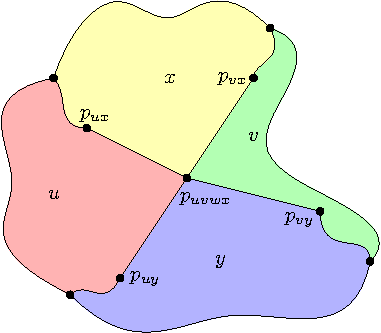
\includegraphics[width=45mm]{Resources/FlipEdge-StretchBoundary-1.pdf}}
	\quad
	\subfigure[]{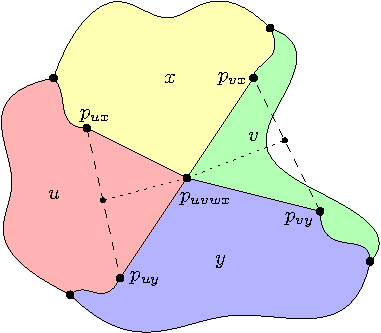
\includegraphics[width=45mm]{Resources/FlipEdge-StretchBoundary-2.pdf}}
	\quad
	\subfigure[]{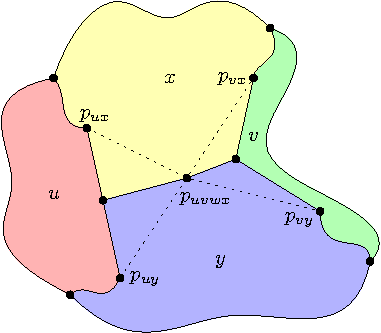
\includegraphics[width=45mm]{Resources/FlipEdge-StretchBoundary-3.pdf}}
	\caption{A contact representation before (a) and after (c) creating a non-degenerate yellow-blue adjacency. (b) shows the construction of potential subdivision vertices.}
	\label{fig:flip-edge-create-boundary}
\end{figure}



\paragraph{Inserting and Removing Edges}

As clusters in our data set grow increasingly similar, we may want to indicate this similarity with new edges between existing clusters in the cluster graph.
Similarly, clusters can grow apart, and we may want to remove edges between clusters in the cluster graph.
However, because the filtered cluster graph is internally triangulated, we cannot insert any more edges on the inside of the graph.
Removing an internal edge is not permitted either, as that would create a hole in the graph.
Consequently, we can insert edges only in the outer face and remove edges only on the outer face.

On top of that, inserting an edge in the outer face is only possible if it preserves the cluster graph's internal triangulatedness.
Therefore, inserting an edge $\{u,w\}$ is only permitted iff $u$ and $w$ lie on the outer face and have a neighbor $v$ in common that also lies on the outer face.
The inserted edge is then embedded such that it forms a new triangular internal face with $v$ and turns $v$ into an internal vertex.
If exactly four vertices bound the outer face before inserting the edge $\{u,w\}$, there exist two candidates for $v$.
In this case, it must be made explicit which one is supposed to become internal and which one is supposed to remain on the outer face.
\Cref{fig:flip-edge-example-insert} shows an example of a valid edge insertion.

\begin{figure}[H]
	\centering
	\subfigure[]{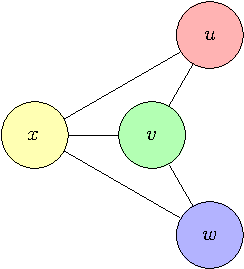
\includegraphics[height=28mm]{Resources/FlipEdge-Example-Insert-1.pdf}}
	\quad
	\subfigure[]{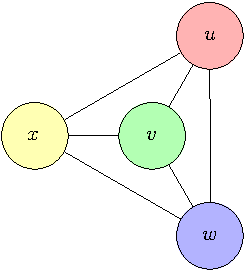
\includegraphics[height=28mm]{Resources/FlipEdge-Example-Insert-2.pdf}}
	\qquad
	\subfigure[]{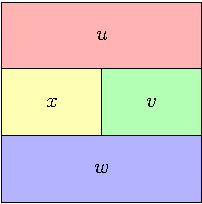
\includegraphics[height=28mm]{Resources/FlipEdge-Example-Insert-3.pdf}}
	\quad
	\subfigure[]{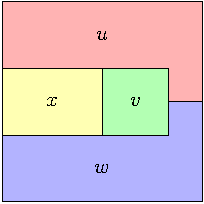
\includegraphics[height=28mm]{Resources/FlipEdge-Example-Insert-4.pdf}}
	\caption{A cluster graph and a polygonal dual thereof, before (a, c) and after (b, d) inserting the edge $\{u,w\}$ to form an internal triangular face with $v$.}
	\label{fig:flip-edge-example-insert}
\end{figure}

Removing an edge $\{u,w\}$ on the outer face of the cluster graph is only permitted if the graph remains biconnected.
This property is preserved iff both $u$ and $w$ have degree $d(\cdot) \geq 3$ and the third vertex $v$ in the internal face bounded by $\{u,w\}$ does not already lie on the outer face.
If that vertex laid on the outer face already, we would end up creating a duplicate adjacency/boundary between $v$ and the outer face, which we specifically excluded in \cref{chap:preliminaries}.
\Cref{fig:flip-edge-example-remove} shows an example of a valid edge removal.

\begin{figure}[H]
	\centering
	\subfigure[]{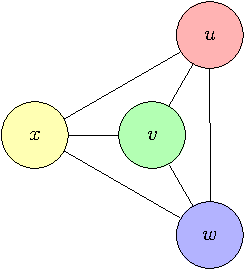
\includegraphics[height=28mm]{Resources/FlipEdge-Example-Remove-1.pdf}}
	\quad
	\subfigure[]{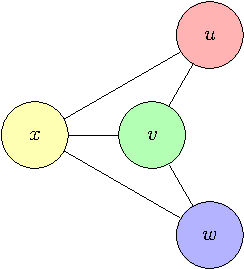
\includegraphics[height=28mm]{Resources/FlipEdge-Example-Remove-2.pdf}}
	\qquad
	\subfigure[]{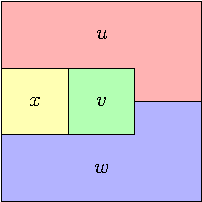
\includegraphics[height=28mm]{Resources/FlipEdge-Example-Remove-3.pdf}}
	\quad
	\subfigure[]{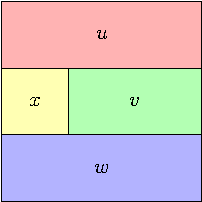
\includegraphics[height=28mm]{Resources/FlipEdge-Example-Remove-4.pdf}}
	\caption{A cluster graph and a polygonal dual thereof, before (a, c) and after (b, d) removing the edge $\{u,w\}$.}
	\label{fig:flip-edge-example-remove}
\end{figure}

Both of these operations are again a special case of the generic edge flip discussed above with a quirk:
Instead of four internal faces, they involve three internal faces and the implicit outer face.

In the example from \cref{fig:flip-edge-example-insert}, we make $v$ into an internal vertex by inserting the edge $\{u,w\}$, removing $v$'s boundary with the outer face in the dual and creating a $u$-$w$-boundary in turn.
Again, recall that in the construction of the augmented dual from \cref{def:augmented-dual}, we insert a helper vertex $v^+$ in the outer face and add edges to all vertices on the original outer face.
This helper vertex and its adjacencies correspond to the outer face and its boundaries in the dual.
When inserting an edge in the outer face, we are essentially flipping the helper edge $\{v,v^+\}$ to become the inserted edge $\{u,w\}$.
Therefore, we apply the same procedure as discussed for the edge flip above, contracting the boundary between $v$ and the outer face into a single point and then creating a non-degenerate $u$-$w$-boundary.

Similarly, when removing an edge $\{u,w\}$ on the outer face as in \cref{fig:flip-edge-example-remove}, a previously-internal vertex $v$ moves onto the outer face.
We can think of it as flipping the edge to be removed to become the helper edge $\{v,v^+\}$.
In the polygonal dual, this gets rid of the $u$-$w$-boundary and creates a boundary between $v$ and the implicit outer face in turn.
Again, we apply the same procedure as discussed for the edge flip, first contracting the $u$-$w$-boundary into a single point and then creating a non-degenerate boundary between $v$ and the outer face.

